This section will describe datasets, baselines, evaluation metrics,
implementation details, and experimental results.

As an implementation-level check of
\cref{thm:appr-star-lower-bound,prop:appr-upper-bound}, we run the reference
APPR implementation on the center-seeded stars
$K_{1,\floor{1/(8\epsappr)}}$ over seven tolerances, four teleportation
parameters, and four legal active-vertex orderings.  Work is measured by the
degree-weighted adjacency-list count $W$ in \cref{eq:appr-work}.  The random
ordering uses seed 17; the other orderings are deterministic.  Every one of
the 112 runs satisfies the proved two-sided interval, as shown in
\cref{fig:appr-star-work-bounds}.

\begin{figure}[t]
    \centering
    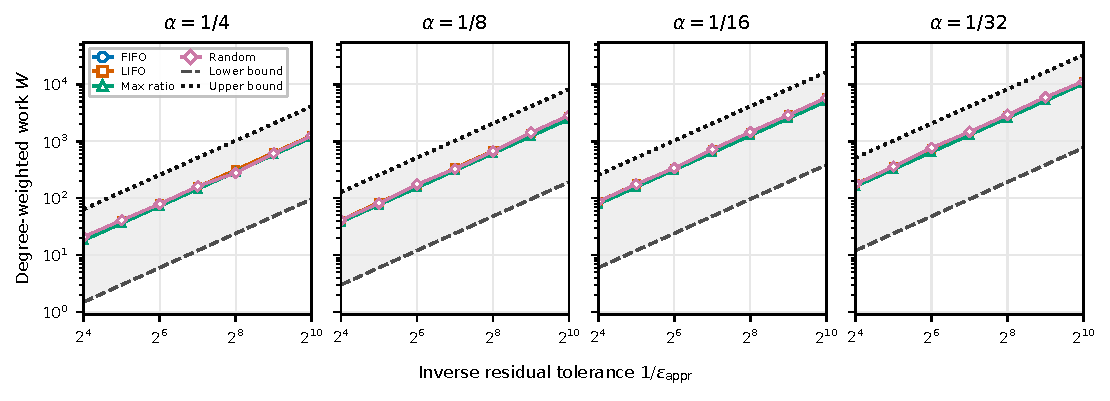
\includegraphics[width=\textwidth]{figures/appr_star_work_bounds.pdf}
    \caption{Actual APPR work on the hard-star construction versus the proved
    lower bound $3/(128\alpha\epsappr)$ and classical upper bound
    $1/(\alpha\epsappr)$.  From left to right, the panels use
    $\alpha\in\{1/4,1/8,1/16,1/32\}$; each varies $\epsappr$ from
    $2^{-4}$ to $2^{-10}$.  The gray region is the theorem interval.  All four
    legal orderings remain inside it; their different costs confirm that the
    guarantee is ordering-independent rather than that every ordering produces
    identical work.}
    \label{fig:appr-star-work-bounds}
\end{figure}
